\section{Results}
\subsection{Mechanical Results}

\subsection{Electrical Results}
Custom Servo motor controllers were developed to fit within the existing footprint of the JX-HV5932MG servos that allowed for position, Velocity and torque control along with live tunable PID, coriolis and gravity gains to allow for smooth control and operation. 

A series of pressure sensing foot sensors were developed to allow for triangulation of the force vector being applied to each foot of the robot. This will allow during future development to determine when and where contact has been made during a step cycle in a gait.

A 9DOF imu board was developed to use the communication protocol of the rest of the robot. By utilizing the BNO055 imu, a number of data sets are able to be collected, the standard sets of gyroscope, magnetometer and accelerometer in X, Y \& Z along with the gravity vector with respect to the IC and the euler angles roll, pitch \& heading. This data will allow for the dynamics of the system to be obtained quickly and accurately to be used in computing the corrective gait cycles.

An integrated charging board that reports the status of the battery pack to the motherboard and in turn motors (for accurate force calculation) was developed in rder to easily charge the battery pack with in the robot at the highest charging current permitted by the specifications of the battery pack and reporting back to the motherboard in order to prvent from over draw of the system, which would result in damage caused to the battery pack. 

The motherboard developed for this robot handles all communication through out the system including communication to and from the motors, IMU, foot sensors and battery charger. The motherboard also handles communication back and forth to the integrated onboard computer through USB HID where all the kinematics and gaits are processed using data from both the updated trajectory pose and the information returned from the system. 

\subsection{Software Results}

\subsection{Overarching Results}
we made a kool robit. look it!
\begin{figure}[H]
            \centering
            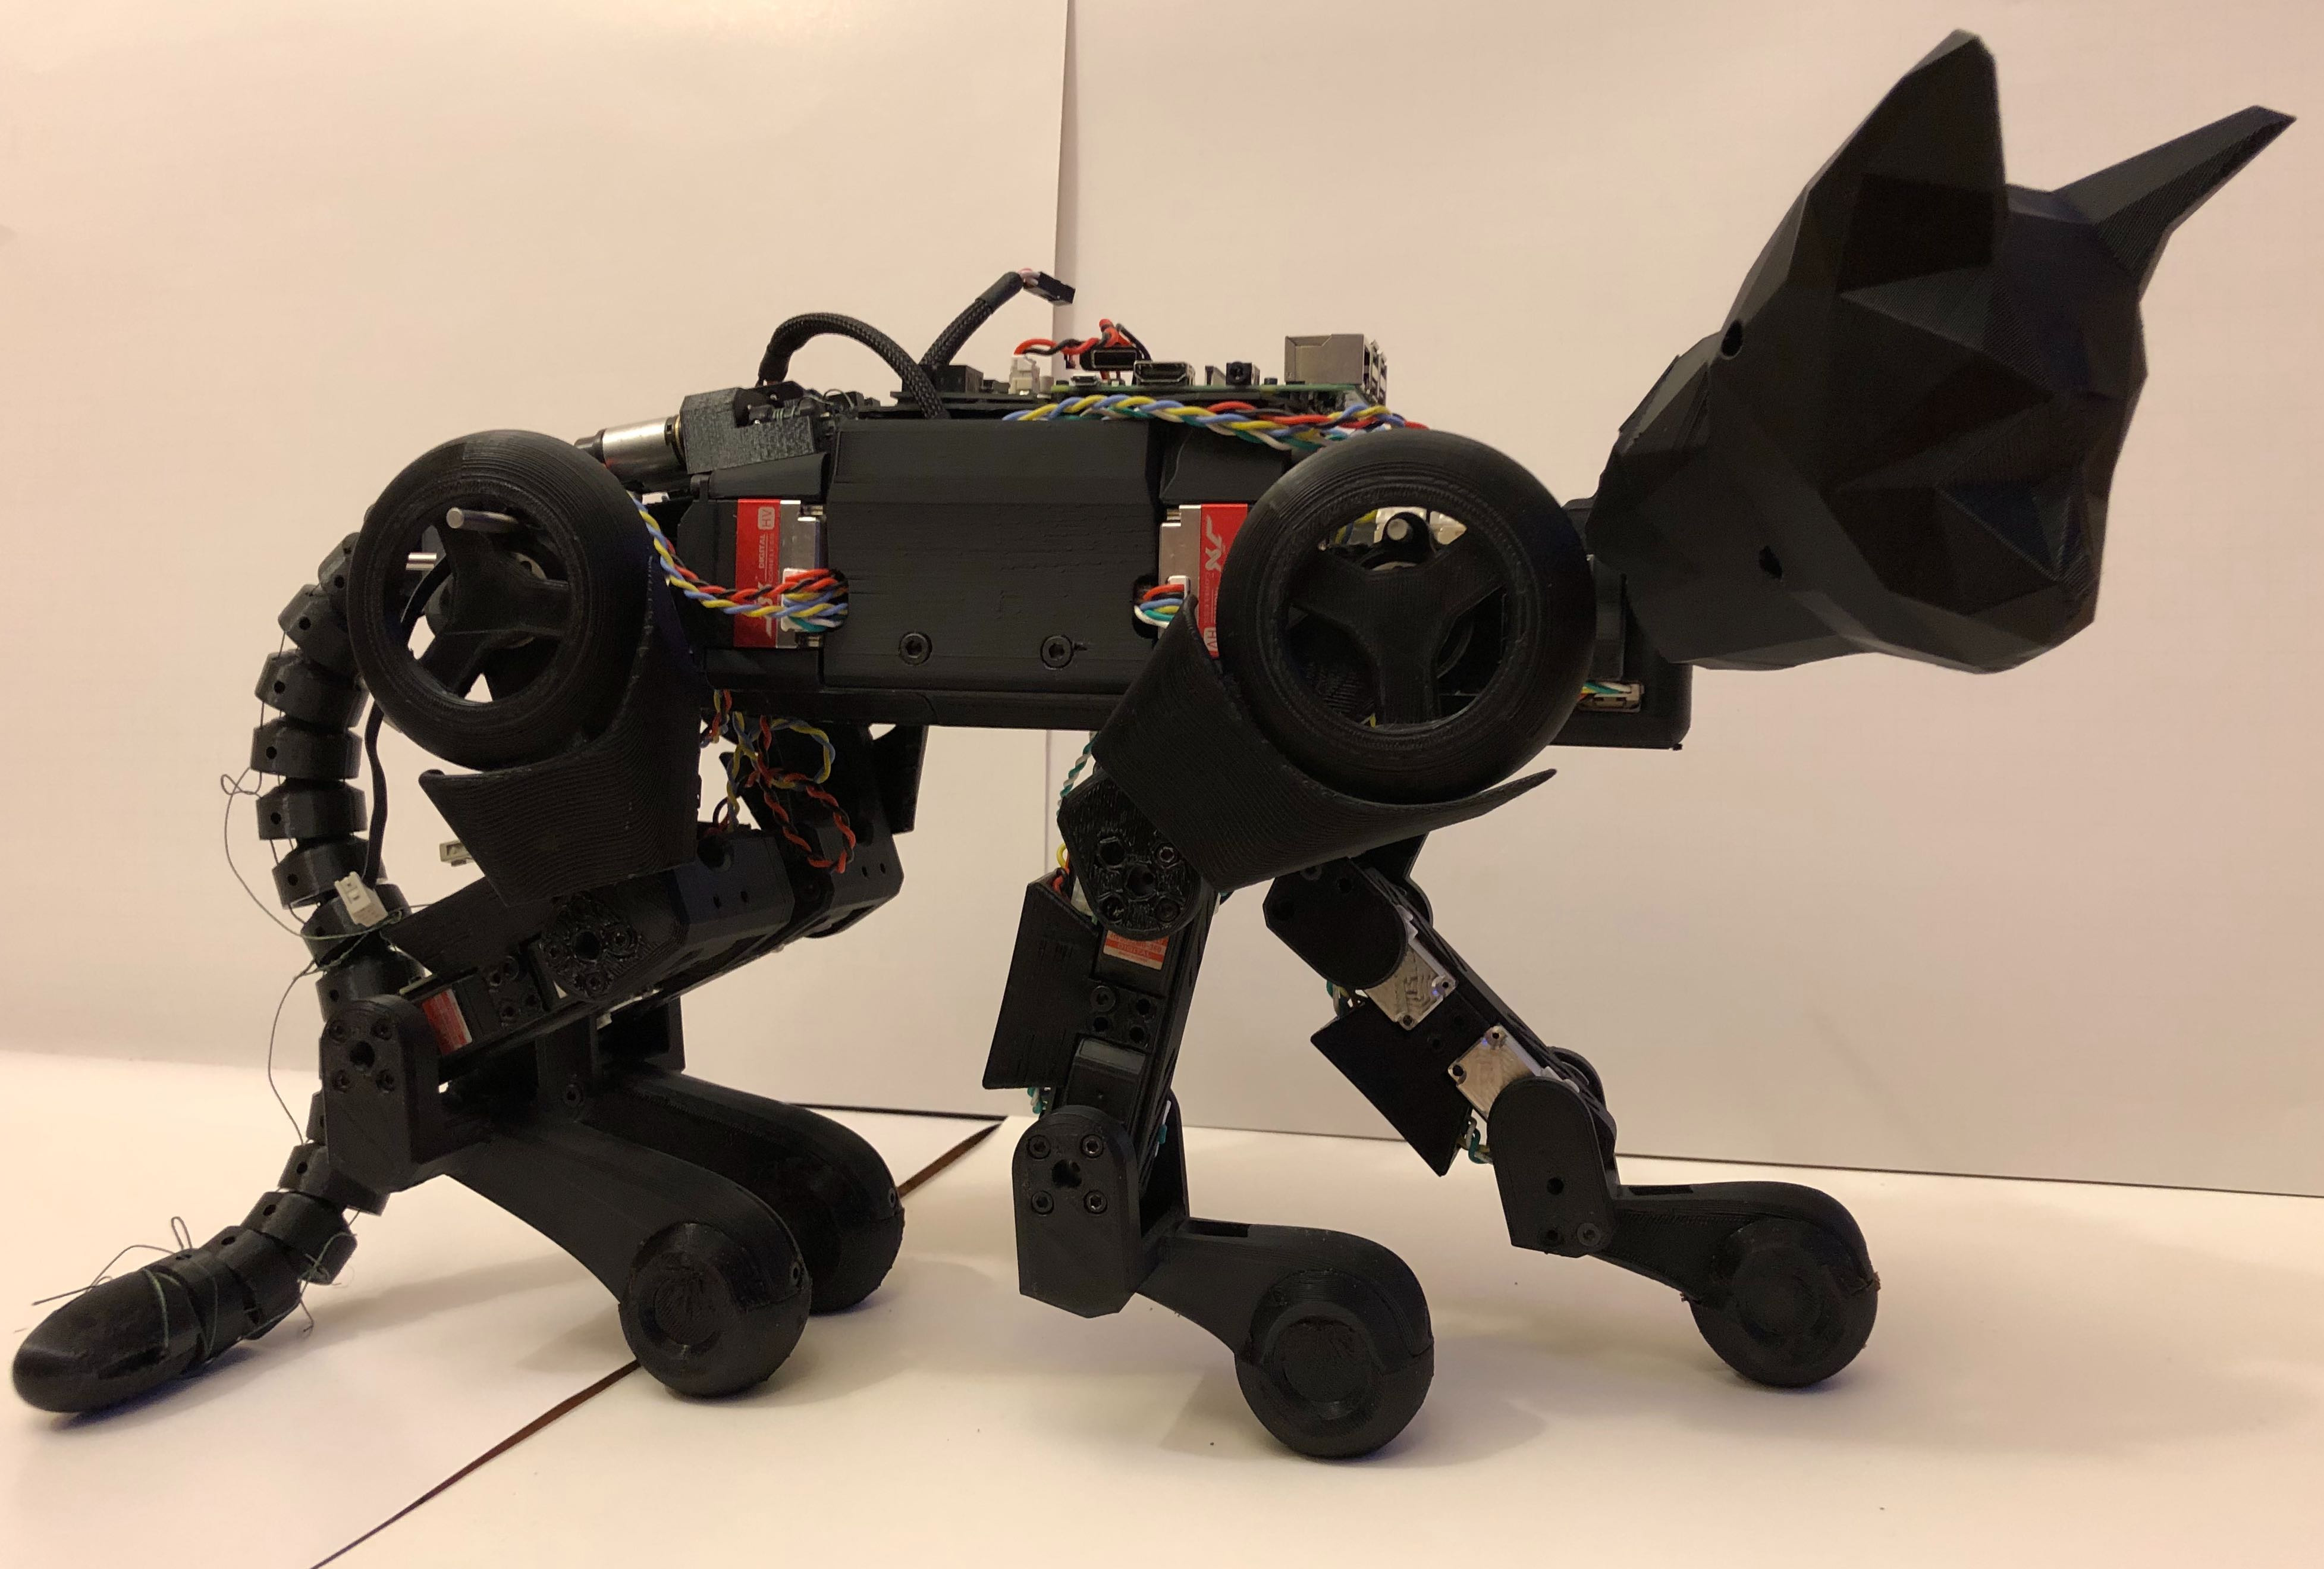
\includegraphics[width=120mm]{figures/FinalRobot.jpg}
            \caption{Final Robot}
            \label{fig:FinalRobot}
        \end{figure}
% Add finished robot picture / rendering in this section
